\cleardoublepage
\chapter{Test av CMS og nettsted}
\label{chap:evaluation} 
% \meta{
% De fleste prosjekter avsluttes med en eller annen form for evaluering av resultatene fra prosjektene. I utviklingsprosjekter vil det være naturlig med teknisk testing, fungerer programvaren som den skal? Teknisk testing kan utføres av utviklerne selv, eller en ekstern part, f.eks. oppdragsgiver. En oppdragsgiver ønsker ofte å utføre en akseptansetest, dvs. en test som vil avgjøre om de har "fått det de har betalt for". Ellers vil det i mange tilfeller være nyttig og viktig med en brukertest, dvs. en strukturert test der sluttbrukerne får komme til orde.

% Evalueringsmetoden vil altså avhenge sterkt av typen av prosjekt. Likevel vil de samme overordnete prinsippene gjelde for alle typer leveranser. En utredning bør kunne passere en akseptansetest, et mediaprosjekt bør kunne underlegges både akseptanse- og brukertest (jfr. kritikerprosessen rundt nye spillefilmer), og et programvareprosjekt bør i tillegg gjennomgå en teknisk test.
% }

I dette kapittelet vil vi gjøre en evaluering av CMS-et og nettstedet som vi har utviklet. Videre vil resultatene fra brukertester, akseptansetest utført av oppdragsgiver og til slutt en teknisk test bli presentert.

\section{Brukertest}
For brukertesten har vi laget forskjellige caser som de forskjellige personene skal gjennomføre. Brukertesten ble gjennomført av 3 personer i ulike aldersgrupper.

\subsection{Caser}

\subsubsection{Case 1}
Du ønsker å lære mer om bedriften og visjonen bak Sirkus Media. Hva gjør du for å løse dette?

\subsubsection{Case 2}
Du ønsker å lære mer om tjenestene til Sirkus Media. Hva gjør du for å løse dette?

\subsubsection{Case 3}
Du ønsker å komme i kontakt med Sirkus Media. Hva gjør du for å løse dette?

\subsection{Valg av testpersoner }
Oppdragsgiver har en ganske bred målgruppe, da de fleste bedrifter ønsker å gjøre markedsføring på nett. Vi ønsket at brukertestene skulle gjenspeile dette. Derfor valgte vi 3 personer i ulike aldersgrupper og med forskjellige forutsetninger når det gjelder til surfing på nettet, til å utføre brukertestene.

\subsection{Testing av nettstedet}
Alle testpersonene gjennomgikk de samme 3 casene i gitt rekkfølge, mens et gruppemedlem observerte.

\subsubsection{Testperson 1}
Testperson 1 var en kvinne på 50 år, som utførte testen på en laptop. Etter at case 1 var opplest, scrollet hun seg først litt rundt på forsiden, før hun tilslutt trykket på menypunktet \q{Om oss}. Her fant hun den informasjonen hun ønsket. Da vi deretter leste opp case 2, klarte ikke vedkommende å ta seg tilbake til forsiden ved hjelp av brukergrensesnittet til siden. Hun endte da opp med å trykke på knappen tilhørende nettleseren for å ta seg tilbake. Etter enda en runde med scrolling på forsiden, oppga hun at i en slik situasjon hadde tatt kontakt gjennom chatten, i steden for å måtte lete etter den informasjonen hun var ute etter. For case 3 trykket hun seg inn på \q{Kontakt oss}-siden og oppga at hun enten hadde brukt kontaktskjema, chatten eller sendt en e-post til adressen som er oppgitt på siden.

\subsubsection{Testperson 2}
Testperson 2 var en mann på 30 år, som gjennomførte testen på mobil. Case 1 ble raskt løst ved å trykke inn på menypunktet \q{Om oss}, som inneholdt informasjonen han ønsket. For case 2 åpnet han først menyen for å se om det var et passende menypunkt her. Da det ikke var det, navigerte han seg tilbake til forsiden og fant frem til den passende informasjonen som befant seg litt lengre ned på siden. På case 3 valgte han å ta kontakt gjennom knappen på forsiden, som fører til kontaktskjema som befinner seg på forsiden. Han oppga også at dersom han ikke hadde tatt kontakt gjennom kontaktskjema hadde han ringt nummeret som ble presentert i headeren. 

\subsubsection{Testperson 3}
Testperson 3 var en kvinne på 25 år, som utførte testen på laptop. Etter å ha fått oppgitt case 1 trykket hun raskt inn på \q{Om oss}-siden og fant frem til teksten som beskrev bedriften. Under case nummer 2 trykket hun seg tilbake til forsiden ved hjelp av logoen. Etter litt scrolling oppga hun at hun også er en slik person som hadde tatt kontakt via chatten, for å få høre mer om tjenestene til bedriften. For case 3 trykket hun seg innpå \q{Kontakt oss}-siden og oppga at hun hadde tatt kontakt gjennom dette skjema, om hun ikke allerede hadde tatt kontakt via chatten. 

\subsection{Evaluering og konklusjon av brukertester}
Etter at alle testpersonene hadde gjennomført de ulike casene kunne vi sette oss ned, gå igjennom testene og komme frem til en konklusjon. Det første interessante funnet var at flere oppga at de hadde tatt kontakt gjennom chatten for å få vite mer om tjenestene til oppdragsgiver. Vi tror grunnen til dette er at ingen av overskriftene eller menypunktene hadde ordet \q{Tjenester} i seg. Likevel tror vi at situasjonen hadde vært annereldes om caset hadde vært reelt og en potensiell kunde hadde ønsket å finne ut mer om tjenestene til Sirkus Media. Vi tror at personen hadde tatt seg tid til å lese gjennom teksten på siden før en eventuell kontakt. Samtidig ønsket vi å gjøre det enda lettere for kundene å finne frem og forbedre brukeropplevelsen. Vi besluttet derfor å legge til et menypunkt som heter \q{Vår prosess} og tar brukeren til informasjonen om prosessen, som også omhandler oppdragsgivers tjenester.

Et annet funn vi gjorde, var at ikke alle klarte å komme seg tilbake til forsiden. Vi bestemte derfor å legge til menypunktet \q{Forside} på alle sider unntatt selve forsiden.

Videre fikk vi også noen tilbakemeldinger på designet. Alle testpersonene mente at siden fremstod som pen og imøtekommende, og at den var generelt var lett å finne frem på. Alt i alt syns studentgruppen at resultatene fra brukertestene var meget positive og samtidig lærerikt.

\section{Akseptansetest}
Etter at første versjonen av nettsted og CMS var ferdig, kunne oppdragsgiver teste systemet. Målet med denne testen var å kartlegge hvor fornøyd oppdragsgiver var med produktet, samt hvilke endringer som burde foretas. I akseptansetesten blir det mulig for oppdragsgiver å verifisere at leveransen er i henhold til bestillingen. 
Etter at versjon 1 ble lastet opp på midlertidig domenet fikk oppdragsgiver beskjed om å teste å prøve å lage en ny side med komponenter og innhold, endre innholdet på eksisterende sider og slette den nyopprettede siden. Før testingen ble det sendt ut brukerveiledning på e-post\footnote{Se vedlegg \ref{appendix:user-manual}}. Oppdragsgiver fikk også beskjed om å gå igjennom de forskjellige sidene og komme med tilbakemelding på designet. 

Vi fikk følgende tilbakemelding på forespørselen vår: 

\begin{quote}
Da har jeg testet ut systemet dere har utviklet. Jeg synes det var veldig enkelt og oversiktlig å gjøre endringer i eksisterende sider i systemet. Det var også veldig enkelt å forstå hvordan man skulle koble opp nye sider til meny etc. Jeg fikk ikke til å lage en fin ny side med fint design slik som dere har gjort, da teksten jeg lagte endte opp helt i hjørnet av siden. Eksisterende tekst og bilder hadde jeg ingen problemer med å endre på.

Når det gjelder design går vi for det dere har laget med noen små endringer om mulig. Er det mulig å endre fonter? Skulle gjerne hatt en litt stiligere font i overskriftene! De kan også være en størrelse større. Da tenker jeg spesielt på «metodene som skaper resultater» og underoverskriftene som tilhører. Jeg synes footeren nederst også kunne vært litt mindre/ smalere. Kunne dere kanskje gjort dette noe mer kompakt? Til sist syns jeg også «resultatene vi har skapt for kundene våre» kunne kommet litt tydeligere frem!

Ellers syns jeg dere har gjort en veldig god jobb, siden ser fresh ut, og vi har med de elementene vi ønsker!
\end{quote}

\subsection{Konklusjon av akseptansetest}
Studentgruppen syns tilbakemeldingen fra oppdragsgiver var meget positiv. Det var et par punkter de ønsket å forbedre på nettstedet, men slikt må regnes med i en slik utviklingsprosess. Alle punktene var også enkle å rette opp i, slik at det ferdige produktet nå er helt etter ønskene til oppdragsgiver. Vi endret fonten til overskrifter og gjorde de større, se figur \ref{fig:typography-new}. I tillegg gjorde vi footeren mer kompakt.
\begin{figure}[H]
    \centering
    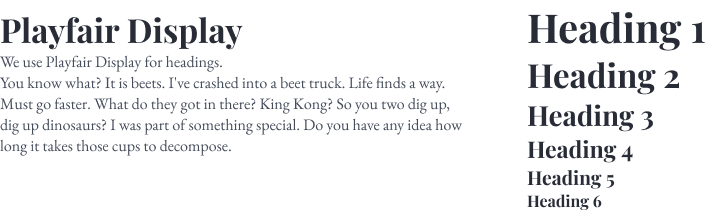
\includegraphics[width=\textwidth]{design/typography-headings.png}
    \caption{Den nye fonten; Playfair Display}
    \label{fig:typography-new}
\end{figure}

Vi besluttet også å oppdatere brukerveiledningen, slik at den inneholdt en oversikt over hva de forskjellige komponentene inneholdt. Her la vi også inn noen tips for hvordan en side kunne opprettes, slik at designet fulgte samme stil som de andre sidene.

Oppdragsgiver fremstod som veldig fornøyd, og vi kan dermed konkludere med at akseptansetesten er godkjent.

\section{Teknisk test}
I dette avsnittet vil vi gjennomføre den samme testen som ble utført i konkurrentanalysen i kapittel \ref{sec:competitor-analysis}. Videre vil vi sammenligne resultatene fra den nye og gamle løsningen. Til slutt vil vi sammenligne resultatene fra den nye løsningen med konkurrentenes resultater. Testene ble gjennomført før chatten ble implementert, og kan derfor avvike noe om de blir kjørt igjen.

\subsection{Testing av ferdig nettsted}
Figur \ref{fig:analysis-new-website} viser det nye nettsted på PC og mobil.

\begin{figure}[H]
    \begin{center}
        \subfigure[PC]{
            \label{fig:analysis-new-website-desktop}
            \frame{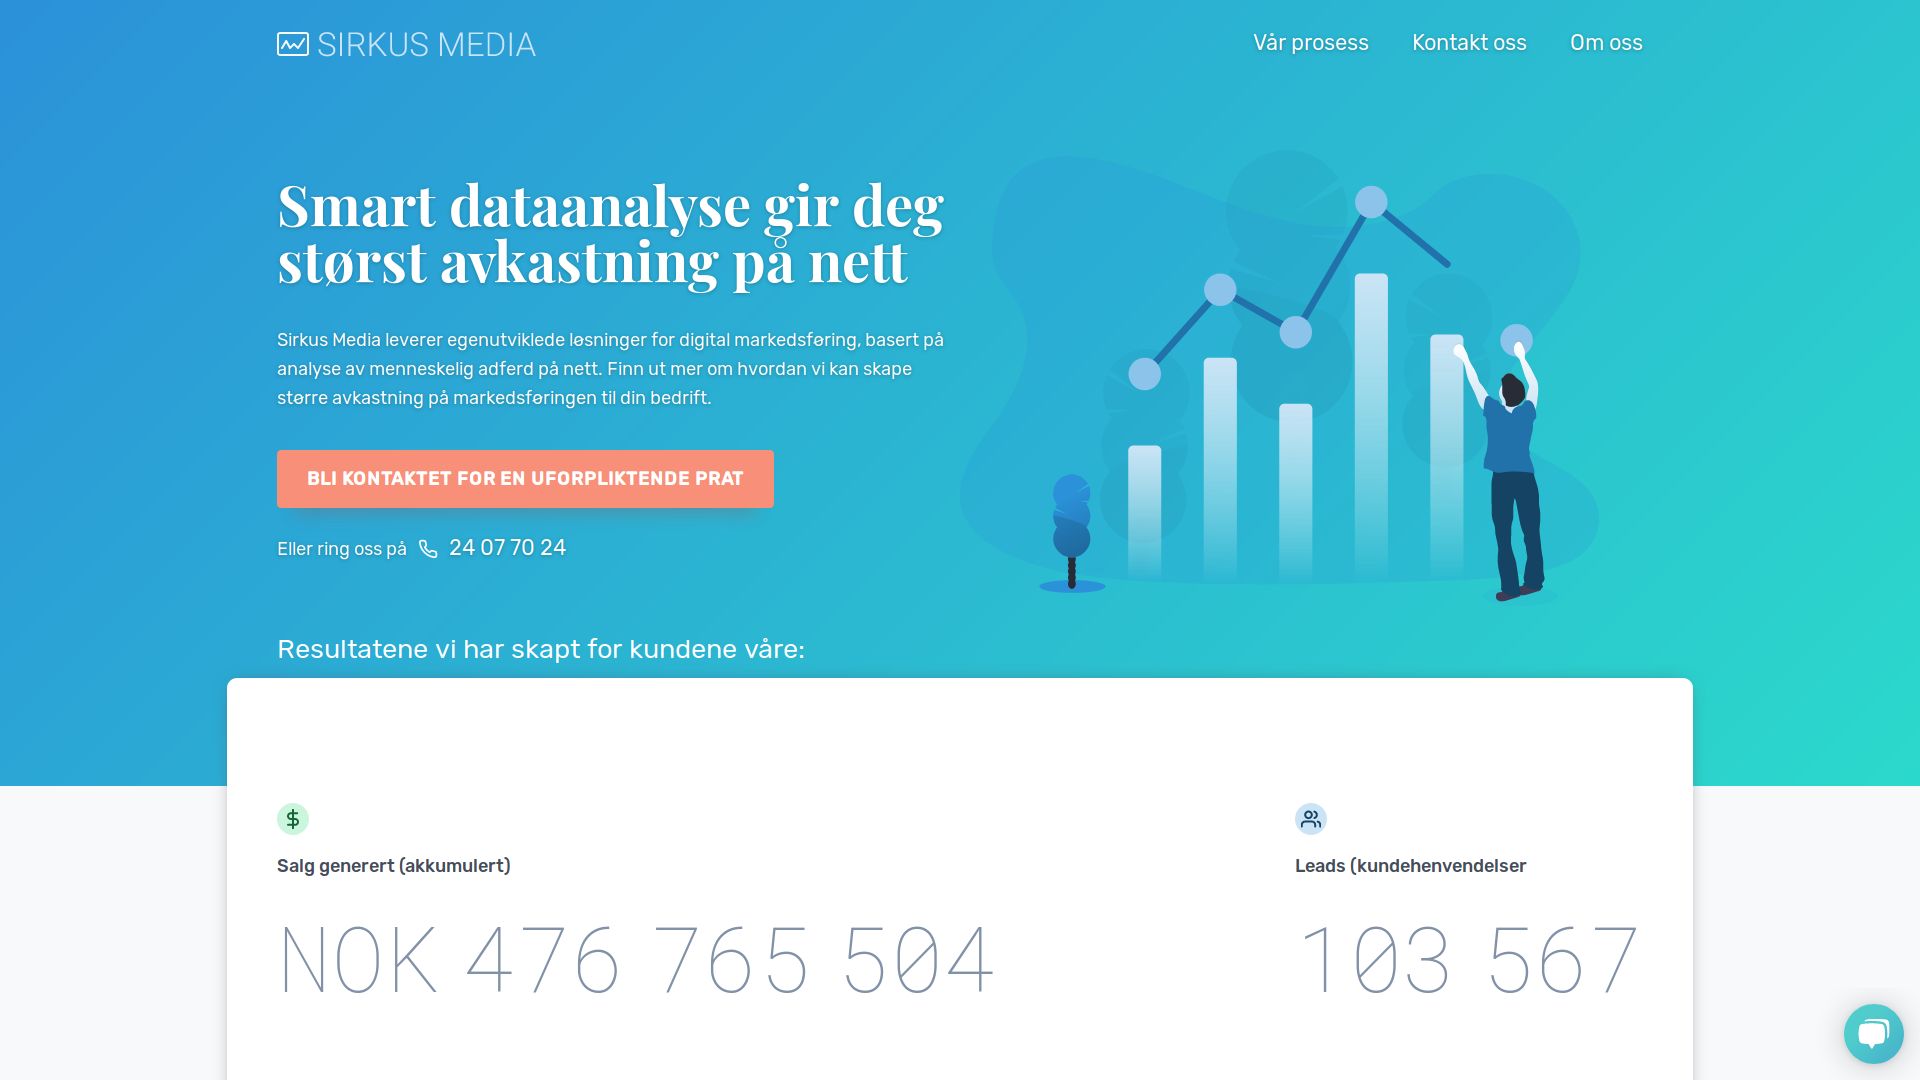
\includegraphics[width=0.71\textwidth]{bjornar/website-new-desktop.png}}
        }
        \subfigure[Mobil]{
            \label{fig:analysis-new-website-mobile}
            \frame{
\includegraphics[width=0.24\textwidth]{bjornar/website-new-mobile.png}}
        }
        \label{fig:analysis-new-website}
        \caption{Nye sirkusmedia.no}
    \end{center}
\end{figure}

\subsubsection{Google chrome Devtools}
Med Google Chrome DevTools testet vi hastigheten til siden. Det ble benyttet et kablet nettverk med hastighet på 100 Mbps. Resultatene måles i millisekunder.

\begin{table}[H]
\begin{center}
\begin{tabular}{lllll}
Test & DOM & Load &  &  \\
1 & 177 & 176 &  &  \\
2 & 177 & 176 &  &  \\
3 & 182 & 182 &  &  \\
4 & 185 & 184 &  &  \\
5 & 179 & 178 &  &  \\
6 & 183 & 182 &  &  \\
7 & 185 & 184 &  &  \\
8 & 181 & 180 &  &  \\
9 & 173 & 173 &  &  \\
10 & 178 & 178 &  &  \\
\end{tabular}
\end{center}
\caption{\label{tab:table-analysis-new-website}Resultater fra hastighetstest med Google Chrome DevTools - Ny løsning}
\end{table}

Gjennomsnitt:\\
- DOM: 180,0 ms\\
- Load: 179,3 ms

\subsubsection{Test med Google Lighthouse}
Videre ble det utført en test ved hjelp verktøyet Google Lighthouse. Figur \ref{fig:analysis-new-lightouse-summary} viser en oppsummering av resultatene. Etter å ha kjørt testen viser det seg at nettstedet får meget gode poengsummer på alle områder. 

\begin{figure}[H]
    \centering
    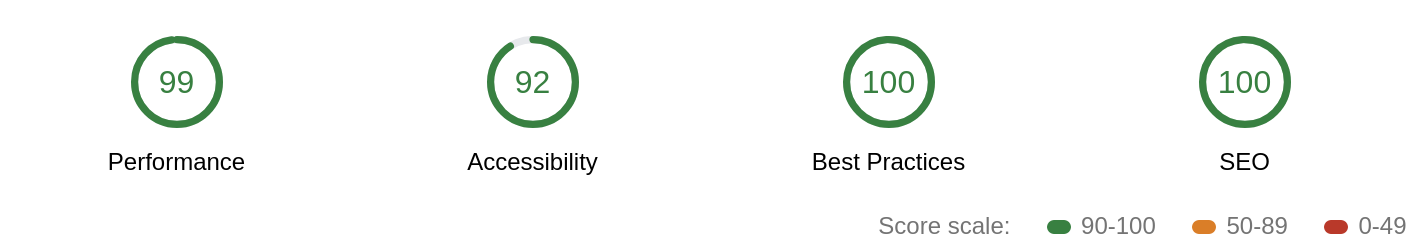
\includegraphics[width=\textwidth]{bjornar/Lighthouse-Report-mobile-new.png}
    \caption{Resultater fra Google Lighthouse - Nytt nettsted}
    \label{fig:analysis-new-lightouse-summary}
\end{figure}

\subsubsection{Checkbot}
Resultatene fra Checkbot viser også en god poengsum i gjennomsnitt. Se figur \ref{fig:analysis-new-checkbot-summary} for resultatene.

\begin{figure}[H]
    \centering
    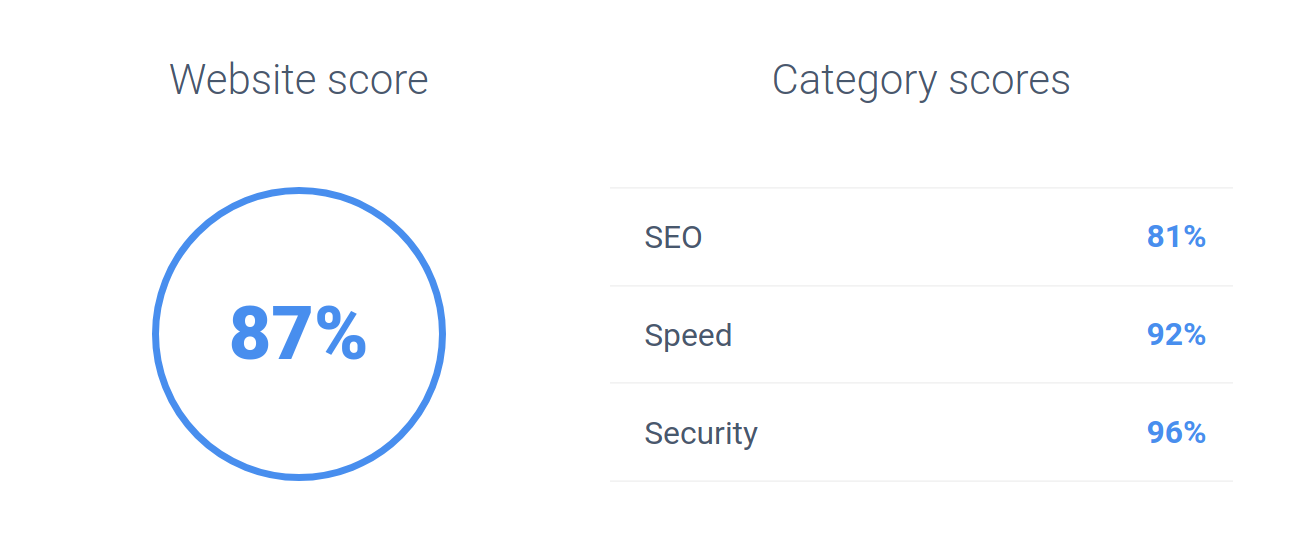
\includegraphics[width=\textwidth]{bjornar/checkbotio-summary-new.png}
    \caption{Resultater fra checkbot - Nytt nettsted}
    \label{fig:analysis-new-checkbot-summary}
\end{figure}

\subsubsection{WAVE \& kontrastforhold}
Ved testing med Wave ble det kun funnet kontrastfeil og noen advarsler. De fleste av kontrastfeilene som blir presentert er ikke reelle, da testen ikke tar hensyn til tekstskygge, noe vi har benyttet oss av nettopp for å få bedre kontrast. Se figur \ref{fig:analysis-new-wave-summary} for resultater. I figur \ref{fig:analysis-new-contrast} ser vi at kontrasten er god nok.

\begin{figure}[H]
    \centering
    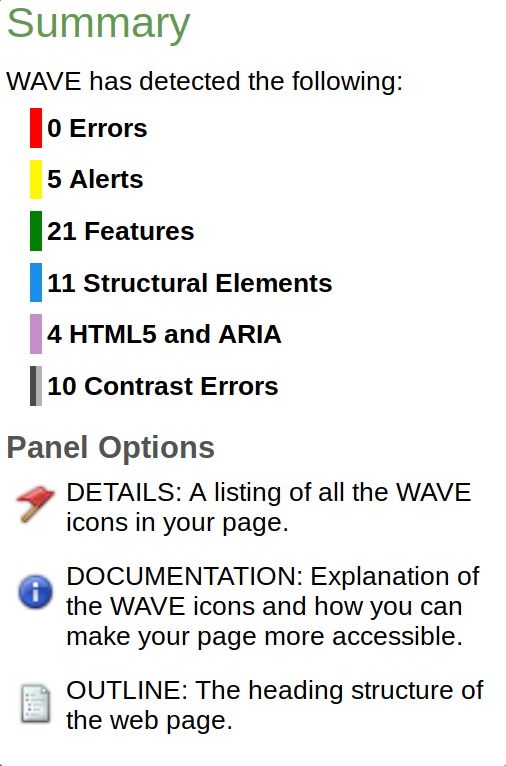
\includegraphics[width=.3\textwidth]{bjornar/wave-new.png}
    \caption{Resultat fra WAVE - Nytt nettsted}
    \label{fig:analysis-new-wave-summary}
\end{figure}

\begin{figure}[H]
    \centering
    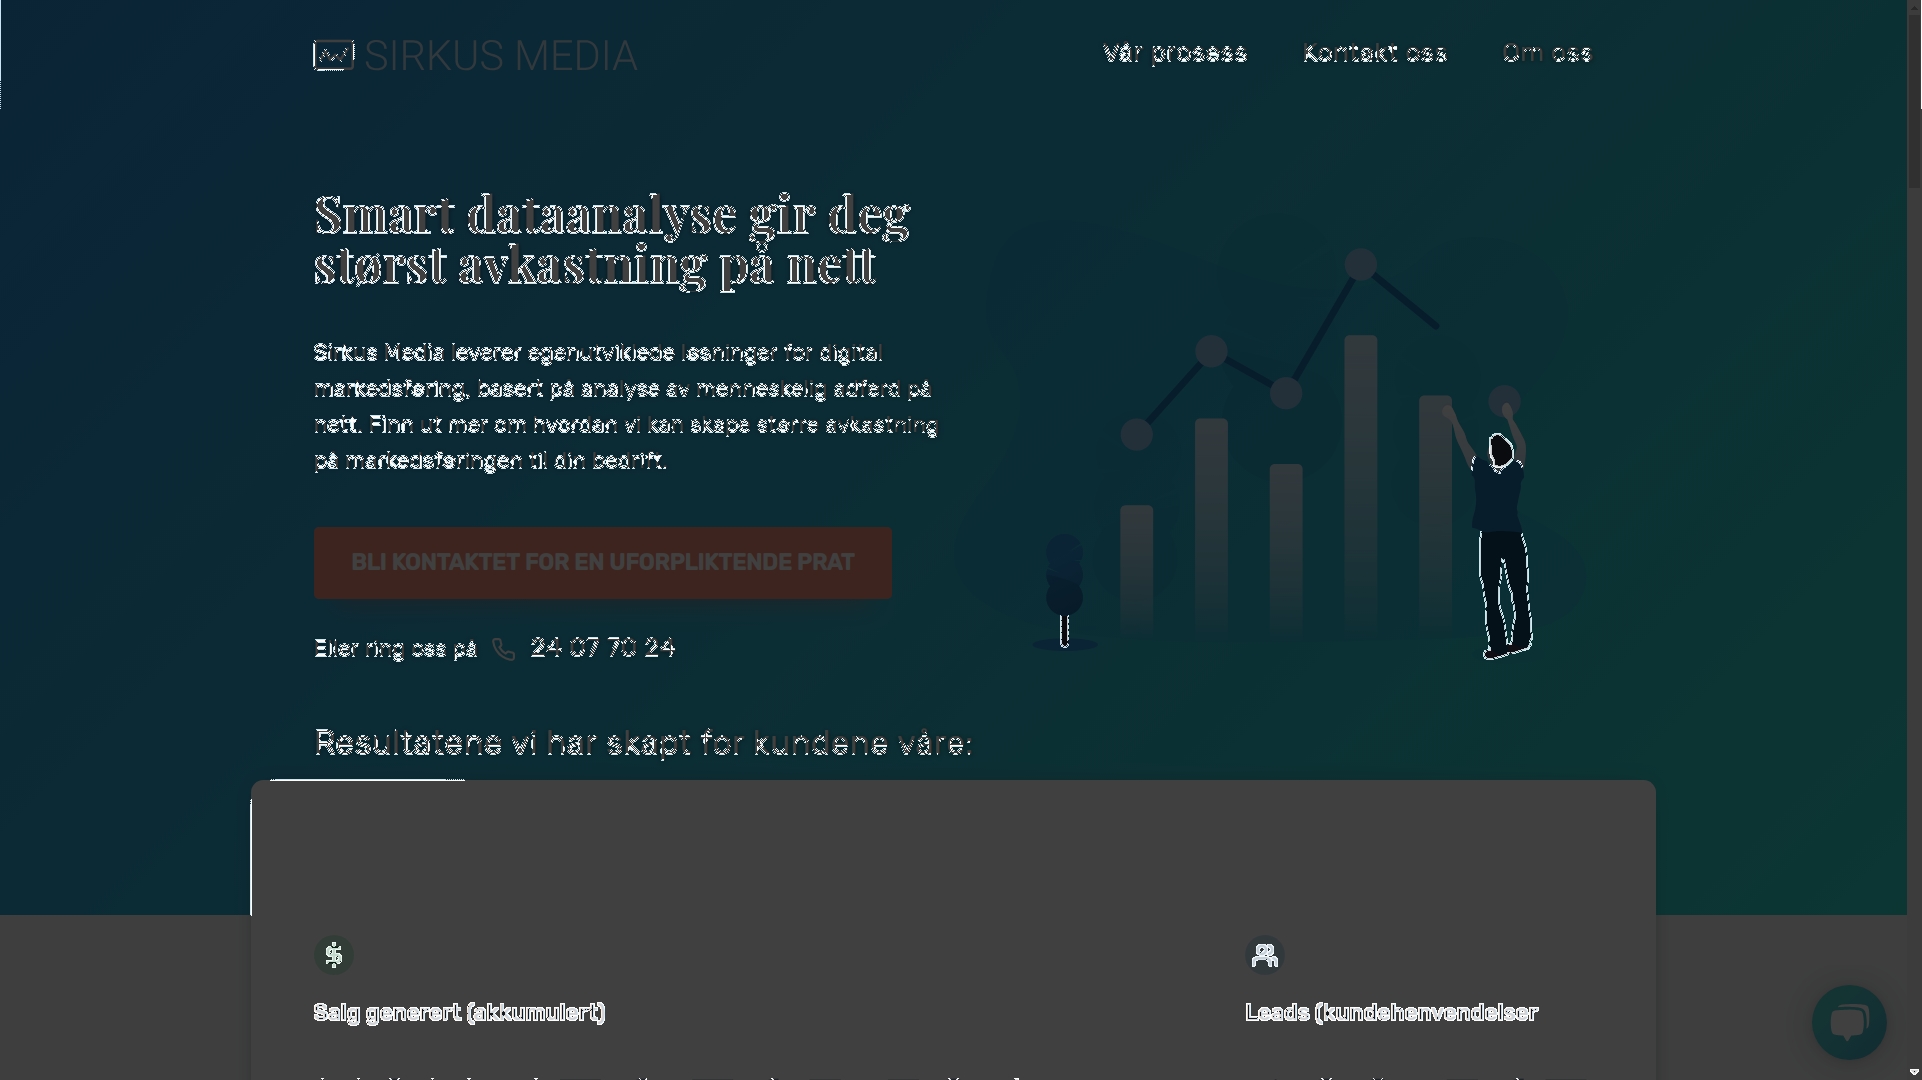
\includegraphics[width=\textwidth]{bjornar/contrast-new.png}
    \caption{Resultat fra kontrast scan med Color Contrast Analyzer - Nytt nettsted}
    \label{fig:analysis-new-contrast}
\end{figure}

\subsubsection{Qualys SSL Server Test}
Resultatet, se figur \ref{fig:analysis-new-ssl-test}, hos Qualys SSL Server ble denne gangen A+. Den har altså blitt forbedret fra en A til en A+.

\begin{figure}[H]
    \centering
    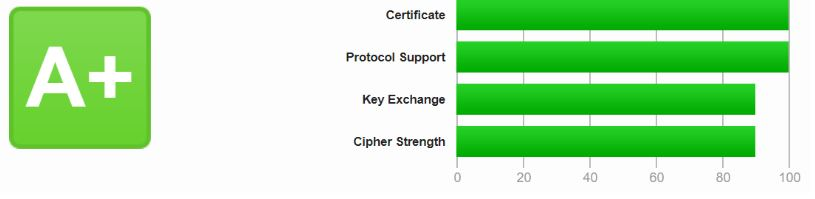
\includegraphics[width=\textwidth]{bereket/QSST-test.png}
    \caption{Sertifikat score - Nytt nettsted}
    \label{fig:analysis-new-ssl-test}
\end{figure}

\subsubsection{Test med skjermleser}
Nettstedet ble også testet med skjermleser. Vi kan konkludere med at det var enkelt å navigere seg rundt på nettsiden fordi innholdet kommer i en logisk rekkefølge. Det har i tillegg blitt lagt til en \q{Hopp til innhold}-knapp som gjør det mulig å hoppe over menyen, som også gjør navigeringen enklere.

\subsection{Sammenligning av ny og gammel løsning}
I avsnitt \ref{sec:analysis-original-website}, der vi analyserte den opprinnelige nettsiden til Sirkus Media, kom det frem via testresultatene at nettsiden var rask. På testen som ble utført på nettet ved høgskolen lastet siden inn på under 1 sekund i gjennomsnitt, noe som var meget bra. Løsningen fikk også 70\% i poengsum hos Checkbot, og jevnt gode resultater i testen gjort med Google Lighthouse. Vi beskrev også hvorfor resultatene ble så gode som de ble. Hovedgrunnen til de gode resultatene var at nettstedet kun bestod av en forside og lite informasjon. Dette begrenset muligheten for feil. Vi hevdet også at det kom til å bli en utfordring å gjøre det like bra i disse testene med et nettsted som består av flere sider, mer innhold og kompleks funksjonalitet.

Når vi nå sammenligner de to løsningene ser vi at nettsiden faktisk har blitt raskere både når det gjelder DOM og Load. Videre ser vi at:

\begin{itemize}
    \item Checkbot fikk 87\% i gjennomsnitt på det nye nettstedet, mens det gamle nettstedet scoret 70\%. 
    \item WAVE kunne ikke rapporterte om noen mangler på det nye nettstedet, men 10 kontrastfeil. Til sammenligning fikk det gamle nettstedet 20 kontrastfeil, 1 mangel, 4 tomme linker og 5 redundante linker.
    \item Qualys SSL Server Test viser A+ på det nye nettstedet og A på det gamle nettstedet.
\end{itemize}

Etter å ha sammenlignet testresultatene mellom den nye og gamle nettsiden, ser vi at den nye nettsiden scorer bedre på alle punkter. Ved testing med Google Lighthouse fikk den nye nettsiden bedre resultat både på ytelse, best praksis, SEO og tilgjengelighet. Kontrastforholdet der elementene ikke bestod testen bør derimot forbedres.

\subsection{Sammenligning av vår løsning mot konkurrentene sine}
I konklusjonen av konkurrentanalysen, avsnitt \ref{sec:analysis-competitors-conclusion}, ble det nevnt at alle konkurrentene hadde bedriftens logo oppe til venstre og et meny ikon til høyre. Vi mente at ved å ha et lignende design på vår løsning, ble det enkelt for brukerne å forstå hvordan menyen fungerer, da denne løsningen er blitt ganske vanlig. Vår løsning endte følgelig opp med et slikt design.

Videre i konklusjonen satte studentgruppen som mål å få minst like bra poengsum på testen til Google Lighthouse som gjennomsnittsscoren til de utvalgte konkurrentene. Den totale gjennomsnittscoren lå på 74,25 av 100 poeng. Vår løsning har en total gjennomsnittscore på 97,75. Vi oppnådde derfor målet vi hadde satt oss.